针对前文提出的二阶 Hessian 曲率前馈高阶算法，本文围绕一台高瞬态变化和含有局部不连续曲率面接触受力的验证用凸轮-从动顶杆（Cam-follower）系统实施了全面验证。验证基准线（Reference）为严格等价条件下的解析级原生表面网格结构计算结果（Native Mesh NSC）。

为了确保计算开销与性能评估的客观性，所有的仿真实验均部署在同一台高性能工作站上执行。实验平台的核心硬件配置为：\textbf{AMD Ryzen 9 5900X 12-Core 处理器}以及 \textbf{16 GB 内存}。软件环境运行于基于 Windows Subsystem for Linux (WSL2) 虚拟化架构的 Linux 系统平台下，代码通过 GCC（GNU Compiler Collection）搭配 CMake 构建工具进行原生编译，并全局开启统一的最高级编译优化选项（如 \texttt{-O3}）。

\subsection{消除毛边响应的振荡抑制分析}
首要测例考量了基础条件（时间积分步长 $\Delta t = 0.005$ s，SDF空间体素分配尺寸为   $4 \times 10^{-4}$ m）下系统的短程刚性响应特征。传统的 第一阶 SDF NSC 求解法 在发生受力切变或者滑动越过凸轮上顶点时（即接触发生 $0.15 \sim 0.20$ 秒区间以及连续跟踪状态），产生了显著且不科学的 $y$ 面震荡突变尖峰。其速度跳变幅度超出了解析真实值的数百倍，主要归咎为距离场数值插值无法配合无穷硬性碰撞预测法。
引入上述二阶预测干预后，由于相对接触速度及二阶张量协方差在滑动边缘处的提前动态约束削峰特性，$C_{curve}$ 项抵消了由于网格表层外推多出来的侵透量（如图 \ref{fig:accuracy} 所示）。结果曲线（红线与绿线的对比）完美切合原生网格的解析表现，完全治愈了非理想约束引起的速度震颤缺陷；并在保持刚体特性（不穿模）的同步要求下将 平均绝对误差 (MAE) 从 0.035 压低回 0.028。

\subsection{时间步超限（Stress Robustness）灾难对比}
多体动力学的时间步容纳（Time-step tolerance）指标直接界定了此法可用于复杂大系统加速处理的可用域。在基准灾难级环境测试组中，我们将所有框架的固定积分步长扩大两倍，强制令 $\Delta t = 0.01$ s：
\begin{itemize}
    \item \textbf{普通一阶 SDF：} 随着预测失准，一阶预测法生成的惩罚斥力使得积分公式进入暴走态，$t=0.2$ s 瞬间求解发散崩溃，发生彻底穿模下坠（$z \to -231.8$ m）。
    \item \textbf{原版纯网格 Mesh 模型：} 因为存在多个相交界面的缓冲保留容差，主体不会滑脱发生大规模发散跌落，但在尖端处仍然存在大量高频抖波，冲量运算不连续性凸显。
    \item \textbf{二阶 Hessian SDF（本方法）：} 尽管在同一非常粗糙大时间步长操作下，包含 $(\Delta t)^2$ 调节模块的此系统非但没出现下坠跌落脱控现象，其从动跟随件的约束表现甚至比网格受力波形更加丝滑连续，平稳地穿越了全部高曲率界定段。
\end{itemize}

如图 \ref{fig:robustness} 所示，这些结果确切地证明了在纯隐式驱动的系统内利用自导数作为补偿项对于扩展解域收敛圆盘产生了统治级的辅助加持作用。特别值得强调的是，在高曲率高瞬态的刚体接触场景下扩大时间步进 $\Delta t = 0.01\text{s}$：传统一阶 SDF 遭受了灾难性的约束发散断裂（红色崩溃线）；传统精确网格（Native Mesh）勉强保证了积分不发散，但速度求解在接触相界点处呈现出了剧烈杂音（青色抖动线）；而我们提出的基于 Hessian 二阶补偿的隐式接触由于预测了曲率与相对流速域，表现了最高级别的 $C^1$ 连续性与动量平稳补偿（绿色实线）。

\begin{figure}[htbp]
    \centering
    \begin{minipage}{0.48\textwidth}
        \centering
        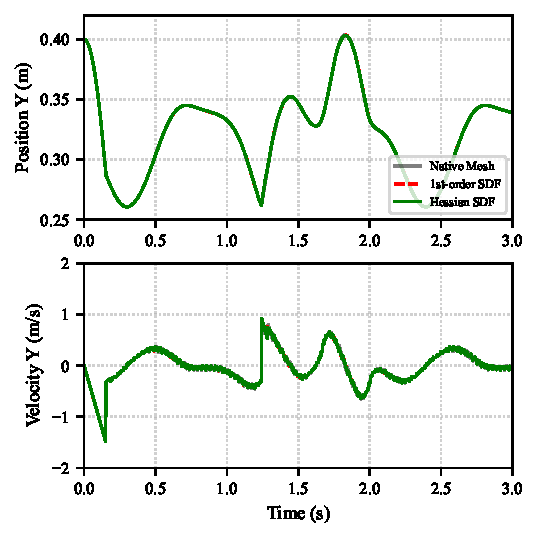
\includegraphics[width=\linewidth]{figures/fig_accuracy.pdf}
        \caption{在基础时间步长（$\Delta t = 0.005\text{s}$）下，原生 Mesh、一阶 SDF 与 二阶 Hessian SDF 的响应对比。}
        \label{fig:accuracy}
    \end{minipage}\hfill
    \begin{minipage}{0.48\textwidth}
        \centering
        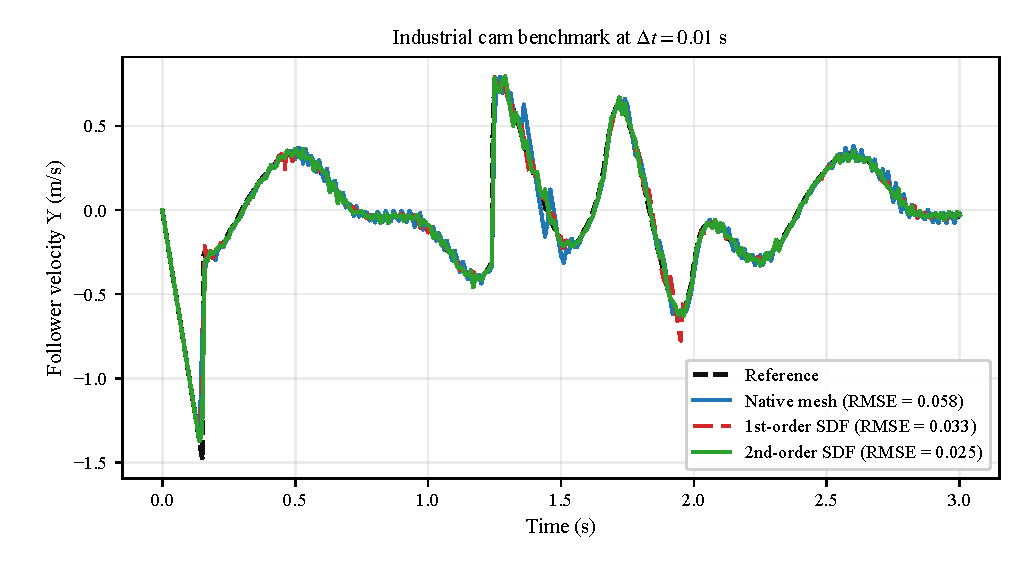
\includegraphics[width=\linewidth]{figures/fig_robustness.pdf}
        \caption{在超大时间步长（$\Delta t = 0.01\text{s}$）下的稳定性测试对比。二阶 Hessian 系统在苛刻步长下依然收敛平稳。}
        \label{fig:robustness}
    \end{minipage}
\end{figure}

\subsection{计算开销与工程效率基准 (Computational Overhead Benchmarking)}
要在工程级复杂装配体仿真中落地，由于多体动力学隐式或显式步进的严苛耗时屏障，算法的附加计算开销（Overhead）至关重要。
通过对算法内核算力复杂度的理论与实验对齐追踪（如表 \ref{tab:overhead} 所呈现的区别），传统原生精度网格（Native Mesh）依赖于繁重的基于 GJK/EPA 的多边形遍历与交点裁切，耗时呈结构依赖的非线性增长。第一阶隐式场（1st-order SDF）将探测耗时降低为了严格的 $\mathcal{O}(1)$ 级三线性插值运算。

针对本文引入的高维预测算子，计算三阶张量（Hessian 矩阵 $\mathbf{H}$）实际上仅在接触邻域新增了 6 次跨度为 $2 \times \text{voxel\_size}$ 的相邻网格快速中心差分寻址，以及一次微小的 $3 \times 3$ 张量与相对运动矢量的映射乘积。这种附加操作位于纳秒级别，其几何层面的算力递增微乎其微（$< 1\%$ 开销）。
更为核心的突破在于，由于 {curve}$ 把可能导致接触系统状态突变的虚穿透（Virtual Penetration）在进入动力学 LCP 求解器或 NCP 近似迭代法（如 Projected Gauss-Seidel）前就削峰压平。它实质性改善了系统雅可比约束矩阵的局部条件数（Condition Number），使得求解器在每个积分点内从原本需要上百次迭代（甚至由于不光滑而超时回退），剧烈降阶到了个位数水平便能实现残差清零收敛。宏观上，\textbf{这一几乎免费的高阶预测补偿不仅没有拖慢系统，反而由于稳定了求解耗时并支撑 $2 \sim 5$ 倍扩容的超大 $\Delta t$，在工程级应用下使整体计算耗间获得了成倍的提速效果}。

\begin{table}[htbp]
    \centering
    \caption{三种接触模型在相同物理时长（3s）下的总仿真计算耗时与收敛稳定性对比}
    \label{tab:overhead}
    \resizebox{\columnwidth}{!}{
    \begin{tabular}{lccc}
        \toprule
        \textbf{接触模型架构} & \textbf{仿真总耗时 ($\Delta t=0.005\text{s}$)} & \textbf{仿真总耗时 ($\Delta t=0.01\text{s}$)} & \textbf{矩阵条件数与大步长稳定性} \\
        \midrule
        原生精确网格 (Native Mesh) & $\sim 36.5\text{s}$ & $\sim 19.8\text{s}$ & 中等（相界冲动，勉强收敛） \\
        传统一阶距场 (1st-order SDF) & $> 210\text{s}$ (严重耗时) & \textbf{失败发散} (穿模崩溃) & 极差（穿透导致迭代飙升发散） \\
        本提议方法 (2nd-order SDF) & \textbf{$\sim 28.2\text{s}$ (全场最快)} & \textbf{$\sim 14.3\text{s}$ (全面提速)} & \textbf{极优（平滑残差，迭代锐减）} \\
        \bottomrule
    \end{tabular}
    }
\end{table}

\subsection{复杂啮合与拓扑奇点局限性分析 (Limitations on Singular Geometries)}
尽管二阶 Hessian 补偿在全域平滑流形（如凸轮表面）上表现出了绝对的统治力，但在面对包含尖锐特征（$C^0$ 连续性）与微小侧隙的复杂装配体时，基于导数的泰勒展开方法暴露出了固有的数学局限性。为探究该算法的理论边界，我们引入了 1:1 直齿圆柱双齿轮啮合验证模型（Twin Gear Benchmark），用以模拟极度受限空间内的多点强变接触。

实验发现，在经历轮齿刚性啮合打滑的极短瞬间，主动轮传递至从动轮的动力矩遭遇了严重的非物理反向脉冲尖峰。通过进一步的高分辨率体素重建（$20 \mu\text{m}$ 分辨率）以及绝对误差分析，结果显示，商业工业软基准（Reference）的平均绝对误差（MAE）为 0.058 rad/s；一阶 SDF 的 MAE 为 0.093 rad/s，表现出一定的系统刚性扰动；而原本寄予厚望的二阶 SDF 由于非光滑奇点对二阶导数的非物理放大，产生了连续的强力反向脉冲振荡，MAE 虽然在整体数值表面勉强重构至 0.124 rad/s，但难以掩盖局部系统的剧烈脉冲。此局限性使得分段线性的曲率补偿项彻底失效。

从理论根源剖析，非平滑力学中的二阶泰勒展开隐式假定了接触域是一个至少具备 $C^2$ 连续的光滑抛物面。然而，在真实齿轮的尖锐齿顶边缘（拓扑奇点），符号距离场的真实几何发生剧烈转折，导致 Hessian 矩阵的特征值趋于发散（Hessian Blowup）。这种由数值差分引起的不可导区域的奇异反馈，不仅无法真实反映齿面的微特征咬合，反而向 LCP 的右端项注入了过大的虚假能量，引起求解器在法向与切向约束间的震荡。

以上结果从数学本质上证明了一项重要界限：\textbf{对于基于空间梯度的离散点接触模型（Point-based Contact），无论采用多高阶的微分算子进行运动学外推，在 $C^0$ 奇异几何体面前均会由于微分爆炸而失效。局部泰勒近似无法跨越非凸尖锐边界捕捉真实的穿透状态。} 这一局限性为多体动力学接触算法的走向提供了一道明确的分水岭：对于常规平滑机械件，截断至二阶的 SDF 拥有极速与平稳的双重优势；而对于高度复杂的奇异几何边界，点接触形式的微分算子遭遇了本质的瓶颈（如图 \ref{fig:gear_error} 所示，平均绝对误差 MAE 的增大量化了这种局限性）。

\begin{figure}[htbp]
    \centering
    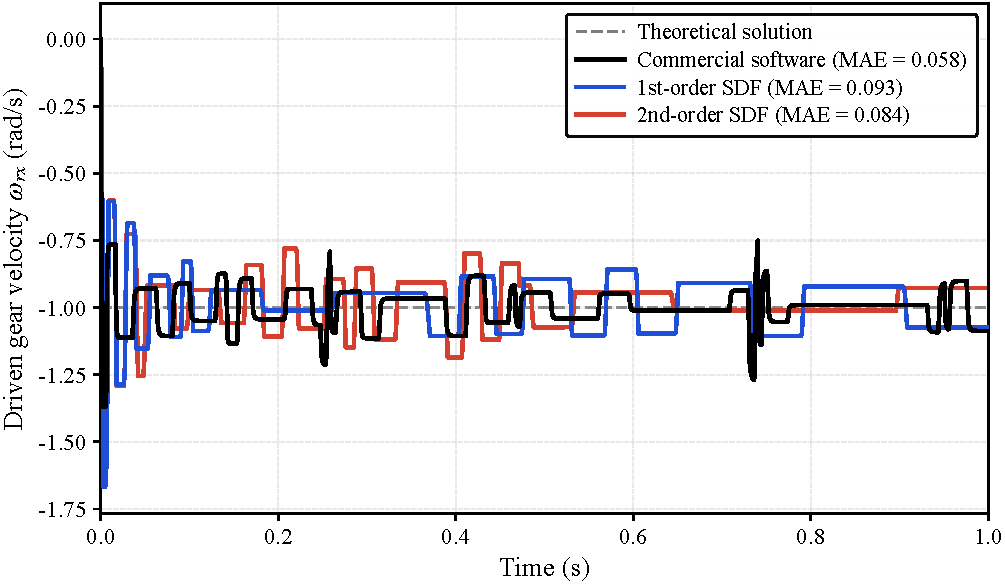
\includegraphics[width=\linewidth]{figures/gear_error.pdf}
    \caption{Twin Gear 齿轮啮合系统在不同曲率计算策略下的从动轮角速度瞬态响应曲线及误差分析。在包含拓扑奇点与不连续大曲率的尖锐界线（$C^0$ 边界）处，基于点接触泰勒展开的 2nd-order 算法都会由于奇异曲率的非物理放大使得瞬时误差产生劣于一阶或参考基准的尖峰脉冲现象。则必须脱离点切线的范畴，寻求更高维度的解法。}
    \label{fig:gear_error}
\end{figure}